\chapter{\label{ch:gnr-hybrid}Graphene Nanoribbons--Metal Porphyrin Hybdrids}

\minitoc

\section{Introduction}\label{gnr-hybrid:sec:intro}

The idea of using chemical functionalisations to induce a preferential doping in carbon nanostructures is not new.
Several proposals have indeed demonstrated the possibility to tune the conductance of ropes~\cite{bockrath2000chemical} and individual~\cite{ zhou2000modulated, ewels2005nitrogen} carbon nanotubes by introducing dopants
in the walled structure, thus leading to $p-n$ junctions and Esaki diodes. These procedures, however, tend to be uncontrolled leaving the substrate with unknown number of dopants per carriers.

In contrast, bottom-up chemical synthesis may provide a viable route to structurally well-defined graphene ribbons with uniform structures in which the dopants are introduced along the edges through control of the chemical functionalisations. Amonngst the various ribbon edges, cove GNRs have attracted a lot of interest for several reasons. First of all, their synthesis can be completely achieved in solution without any surface-assisted methodolgy. Secondly, the steric tension induced by the lateral groups on the structure makes them typically non-planar, open up possibility to investigate not only optical properties but also spin--orbit coupling effects in carbon nanostructures, which have remained so far elusive from experimental evidence.

Furthermore, theoretical calculations have shown that the wave functions for the frontier crystal orbitals are fully delocalized across the ribbon width, in contrast to zigzag-GNRs (with localized states at the ribbon edges), with electronic band gap of cove-edged GNR infinite ribbon settling around 1.70 eV, and mobilities values in the order of thousands \si{\cm\square\per\V\per\second} for both electrons and holes~\cite{Liu2015}.

\section{Chemical Doping MGNRs}
One of the major appeal of \glspl{GNR} is that thanks to the bottom-up synthesis substitutional doping, i.e. the substitution of carbon atoms in the  by , would allow to chemically control electronic properties at a very fundamental level, overcoming a major limitation of the solid-state semiconductors.

When atoms with different number of valence electrons are introduced in the graphene nanoribbon's honeycomb lattice, a charge transfer will occur based on the relative position of the Fermi level of the GNR with the HOMO and LUMO of the dopant atom. For example, if the HOMO of a dopant is above the Fermi level of GNR, a charge transfer will occur from the dopant to the ribbon, and the dopant acts as a donor; if the LUMO is below the Fermi level of GNR, a charge transfer in opposite direction will lead the dopant  to act as an acceptor.

Graphene can be p-type or n-type doped via chemical doping. p-Type doping drives the Dirac points of graphene above the Fermi level, and n-type doping drives the Dirac points below the Fermi level. Generally speaking, molecules with electron withdrawing groups adsorbed on the surface of graphene will lead to p-type doping of graphene, and molecules with donating groups will lead to n-type doping. In contrast, the mechanism of substitutional doping still remains uncertain. p-Type doping is generally achieved by adding atoms with fewer valence electrons than carbon like boron, while n-type doping is generally achieved by adding atoms with more valence electrons than carbon like nitrogen.

In this chapter, we study the effect of introducing several chemical functionalisations from a theoretical and experimental perspective. The experimental results will be

\begin{figure}[hbtp]
    \begin{center}
        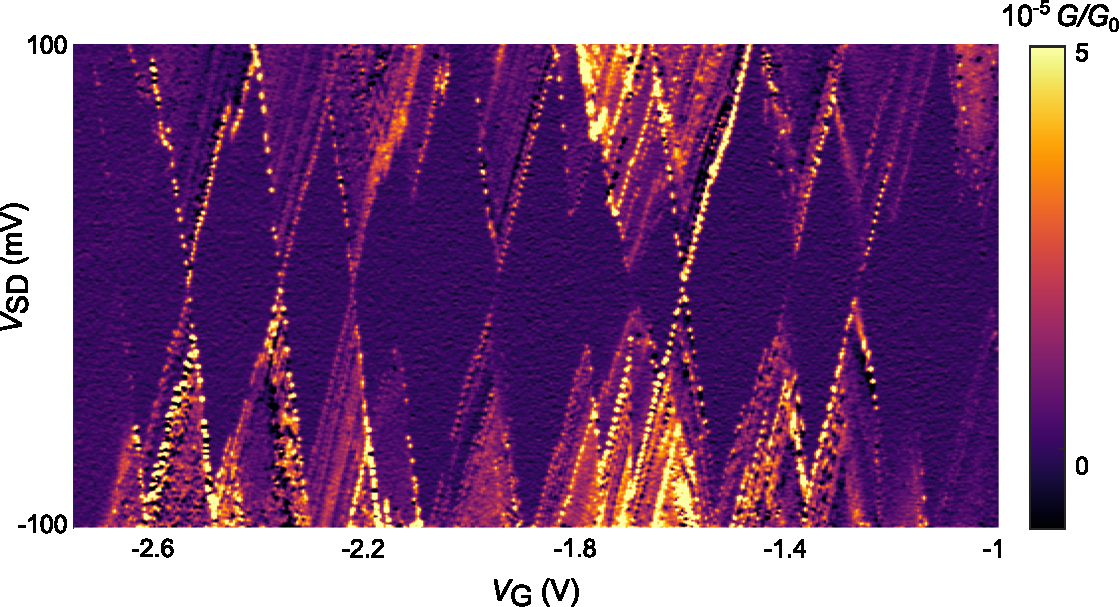
\includegraphics[width=\textwidth]{chapter_thermoelectric/figures/gnr-hybrid.pdf}
        \caption{Stability diagram of gnr-Ni-hybdrid}
        \label{fig:gnr-Ni-hybdrid-sd}
    \end{center}
\end{figure}


\section{Substitutional Doping: Theoretical Modelling}\label{gnr-hybrid:sec:chem_doping}

Collaborators from the Feng group in Dresden and the M{\"u}llen group in Mainz provided graphene nanoribbons with different functional groups along the edges. These ribbons share the same aromatic core and have widths ranging from $w_\textrm{GNR}\simeq$\SIrange{1.1}{1.2}{\nano\metre} with lengths which follow a gaussian distribution (Fig.~\ref{fig:chem_doping:base_ribbon_length_distribution}). This last point comes from that the separation between ribbons having different length is carried out by size-exclusion chromatography means, where the average residence time in the pores created by the column packing depends on the effective size of the analyte molecules. \Glspl{GNR} larger than the average pore size of the packing are excluded and thus suffer essentially no retention; such species are the first to be eluted and are ribbons with longer lengths. On the other hand, ribbons having diameters significantly smaller than the pores may penetrate or permeate throughout the pore network and are thus retained inside the column for the greatest time.

\begin{figure}[hbtp]
    \begin{center}
        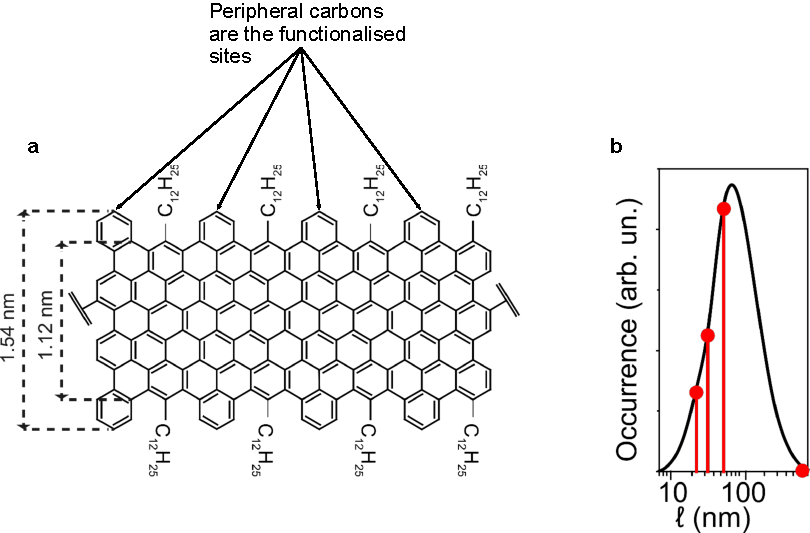
\includegraphics[width=\textwidth]{chapter_thermoelectric/figures/base_ribbon_length_distribution.pdf}
        \caption[Cove-4 GNR structure and Length Distribution]{\textbf{a,} Structure of a 4-Cove graphene nanoribbon. Highlighted are the carbon sites where dopant atoms are introduced through chemical synthesis. \textbf{b,} Distribution of MGNR lengths $l$ as obtained from size-exclusion chromatography on the polymerized molecular precursor (black). Red dots and vertical lines identify various length obtainable with different elution curves. Adapted from~\cite{dotti2018phd}.}
        \label{fig:chem_doping:base_ribbon_length_distribution}
    \end{center}
\end{figure}

Unfortunately these ribbon featured very poor solubility, even after several sonication and dilution cycles in most of the common organic solvents. Since it was not possible to carry out a thorough experimental study at the device level, we have investigated  the structural and electronic properties of GNR-H and compared them with the ones of GNR-OMe, GNR-Br, GNR-Cl, and GNR-Anthracene through DFT simulations.

\begin{figure}[hbtp]
    \begin{center}
        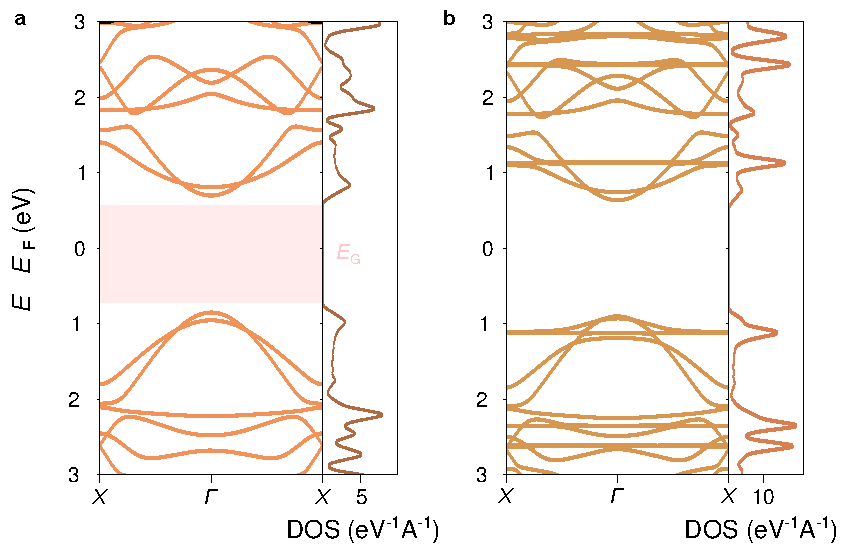
\includegraphics[width=\textwidth]{chapter_thermoelectric/figures/anthracene.pdf}
        \caption[Band structure for a 4-Cove GNR with and without Anthracene]{\textbf{a,} Band structure and density of states for a 4-Cove GNR-H and \textbf{b,} a 4-Cove GNR-anthracene calculated at the DFT-GGA level.}
        \label{fig:chem_doping:base_anthracene}
    \end{center}
\end{figure}

Ab-initio calculations were performed using the package Siesta \cite{soler2002siesta, garcia2020siesta} and testing functionals both within the \gls{LDA} and PBE \gls{GGA}. To simplify the geometry, alkyl chains were removed and replaced with hydrogen atoms. Sufficient vacuum distance is added along the non-periodic directions to avoid unwanted interactions. Numerical atomic pseudopotential was used together with an energy cut-off of 400 Ry. Monkhorst Pack k-point-grid was chosen to be ($20\times 1\times 1$) along the three Cartesian directions. The structure is optimized until the maximum force on the atoms is less than 0.01 eV/Å \SI{0.01}{\electronvolt\per\angstrom}.

\begin{figure}[hbtp]
    \begin{center}
        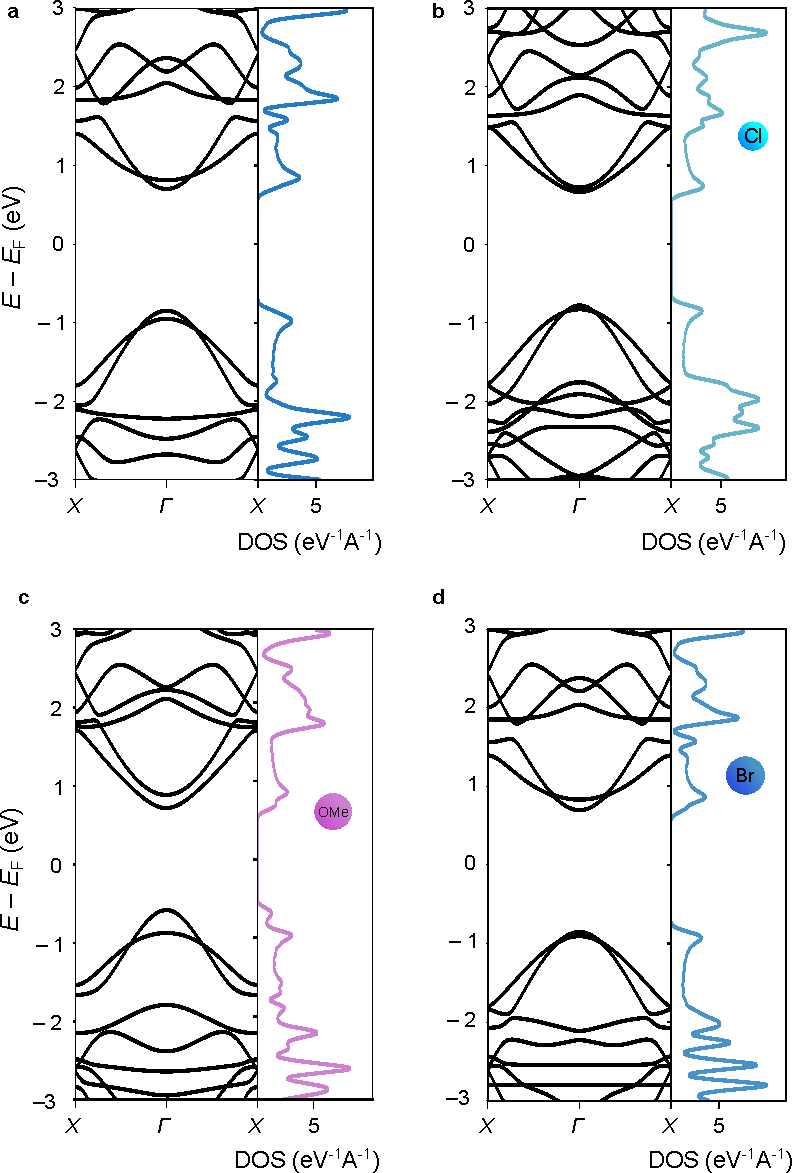
\includegraphics[width=\textwidth]{chapter_thermoelectric/figures/drawing.pdf}
        \caption{Band structure and density of states for graphene nanoribbons decorated with various electron donors or acceptors resulted after applying the GGA approximation for the exchange--correlation energy term.}
        \label{fig:bandstructure_chem_doping}
    \end{center}
\end{figure}

Fig.~\ref{fig:chem_doping:base_anthracene} shows the comparison between the base case and the same ribbon functionalised with anthracene along the edges. Compared to the base case, the introduction of anthracene groups introduces sharpe features in the \gls{DOS} in correspondence of flat lines in the band structure, which may are attributable to a more kind of discrete spectrum. This observation is in agreement with predictions at the \gls{NEGF} level and known as even--odd conductance effect~\cite{vcercnevivcs2020even}. In particular, for functional groups with an odd number of rings, the local density of states resides on the site of the guest molecule which is bound convalently to the nanoribbon, resulting in a non-negligible interaction between the continuum of states in \gls{GNR} and the localised state on the edge-attached adduct.

Furthermore, at this level of theory it appears that the when anthrance groups are introduced along the edges the particle-hole symmetry is broken, as the band structure  spectrum is no longer symmetric with respect to the Fermi energy



Fig.~\ref{fig:bandstructure_chem_doping} compares the band structures and \gls{DOS} between GNR-H (top-left) and other chemical dopants. In the case of GNR-OMe, four electron-donating methoxy groups per repeating unit have been considered, while six negative inductive Clorine groups were considered for GNR-Cl. Firstly, it is possible to observe the frontier bands in case of GNR-OMe are $\simeq\SI{0.5}{\electronvolt}$ higher than those of GNR-H, likely due to charge redistribution induced by the methoxy groups.

In addition to this, the DFT simulations suggests that the aromatic structure of GNR-OMe might be slightly distorted becuase of the steric repulsion introduced by the methoxy groups. In order to test this hypothesis, we performed a DFT simulation of a non-planar GNR-H having the same spatial distortion of GNR-OMe without the methoxy groups. The methoxy groups were replaced by hydrogen atoms after the geometric optimization of GNR-OMe, while keeping the distorted aromatic core fixed. The results suggests that the geometric distortions are responsible for only one-half of the bandgap shrinkage, i.e. \SI{125}{\milli\electronvolt}, while the other half can be ascribed to the larger effective width of the $\pi$-conjugated system of GNR-OMe due to the delocalization of the frontier states over the oxygen of the methoxy groups.

Interestingly, despite the fact that both the Bromide and Chlorine substitutions share electrons with the ribbon preferentially via $\sigma$-bond, GNR-Cl exhibits a more pronounced bandgap contraction (Tab.~\ref{tab:bandgaps}) and a decrease in effective mass $m^*$ at the $\Gamma$ point of the conduction band. The same holds true for the case of methoxy substitution. As the effective mobility $\mu_\textrm{eff}$ of charge carriers is proportional to the inverse of their effective mass, a decrease in the effective mass of the charge carriers may be advantageous for their transport, possibly resulting in better device performance. On the other hand, no appreciable deviation from the base case is observed for the ribbon functionalized with Br groups, which could be explained by a lower electronegativity and consequently a lower ability to induce charge rearrangement of the ribbon's frontiers orbital.



% explain the doping shift from normal n for the Cl and Br to p for methoxy



\begin{table}
    \caption{\label{tab:bandgaps}
        Bandgap values calculated for various chemical substitutions on a 4-cove \gls{GNR}. Exchange-correlation energy is tested within the two main approximation LDA and GGA.}
    \[
        \begin{array}{lcc}
            \hline\textit{Edge}        & \textrm{LDA}         & \textrm{GGA}                                     \\
            \textit{functionalisation} & (\si{\electronvolt}) & (\si{\electronvolt})                             \\
            \hline
            \text{Pure 4-Cove}         & 1.58                 & 1.55                                     \Tsmall \\
            \text{Anthracene}          & 1.56                 & 1.54                                             \\
            \text{-Br}                 & -                    & 1.55                                             \\
            \text{-Cl}                 & 1.45                 & 1.44                                             \\
            \text{-OMe}                & 1.32                 & 1.30                                             \\
            \hline
        \end{array}
    \]
\end{table}



\section{Electrical Transport Measurements}\label{gnr-hybrid:sec:measure}

Explain how the calculations have initially suggested the comparison between the base case and the methoxy groups,
as they have the largest badgap distance.

\section{Concluding Remarks}\label{gnr-hybrid:sec:summary}


\section{Project Overview}